% Options for packages loaded elsewhere
\PassOptionsToPackage{unicode}{hyperref}
\PassOptionsToPackage{hyphens}{url}
\PassOptionsToPackage{dvipsnames,svgnames,x11names}{xcolor}
%
\documentclass[
  12pt,
  letterpaper,
]{book}

\usepackage{amsmath,amssymb}
\usepackage{iftex}
\ifPDFTeX
  \usepackage[T1]{fontenc}
  \usepackage[utf8]{inputenc}
  \usepackage{textcomp} % provide euro and other symbols
\else % if luatex or xetex
  \usepackage{unicode-math}
  \defaultfontfeatures{Scale=MatchLowercase}
  \defaultfontfeatures[\rmfamily]{Ligatures=TeX,Scale=1}
\fi
\usepackage{lmodern}
\ifPDFTeX\else  
    % xetex/luatex font selection
\fi
% Use upquote if available, for straight quotes in verbatim environments
\IfFileExists{upquote.sty}{\usepackage{upquote}}{}
\IfFileExists{microtype.sty}{% use microtype if available
  \usepackage[]{microtype}
  \UseMicrotypeSet[protrusion]{basicmath} % disable protrusion for tt fonts
}{}
\makeatletter
\@ifundefined{KOMAClassName}{% if non-KOMA class
  \IfFileExists{parskip.sty}{%
    \usepackage{parskip}
  }{% else
    \setlength{\parindent}{0pt}
    \setlength{\parskip}{6pt plus 2pt minus 1pt}}
}{% if KOMA class
  \KOMAoptions{parskip=half}}
\makeatother
\usepackage{xcolor}
\usepackage[margin=1in]{geometry}
\setlength{\emergencystretch}{3em} % prevent overfull lines
\setcounter{secnumdepth}{-\maxdimen} % remove section numbering
% Make \paragraph and \subparagraph free-standing
\makeatletter
\ifx\paragraph\undefined\else
  \let\oldparagraph\paragraph
  \renewcommand{\paragraph}{
    \@ifstar
      \xxxParagraphStar
      \xxxParagraphNoStar
  }
  \newcommand{\xxxParagraphStar}[1]{\oldparagraph*{#1}\mbox{}}
  \newcommand{\xxxParagraphNoStar}[1]{\oldparagraph{#1}\mbox{}}
\fi
\ifx\subparagraph\undefined\else
  \let\oldsubparagraph\subparagraph
  \renewcommand{\subparagraph}{
    \@ifstar
      \xxxSubParagraphStar
      \xxxSubParagraphNoStar
  }
  \newcommand{\xxxSubParagraphStar}[1]{\oldsubparagraph*{#1}\mbox{}}
  \newcommand{\xxxSubParagraphNoStar}[1]{\oldsubparagraph{#1}\mbox{}}
\fi
\makeatother


\providecommand{\tightlist}{%
  \setlength{\itemsep}{0pt}\setlength{\parskip}{0pt}}\usepackage{longtable,booktabs,array}
\usepackage{calc} % for calculating minipage widths
% Correct order of tables after \paragraph or \subparagraph
\usepackage{etoolbox}
\makeatletter
\patchcmd\longtable{\par}{\if@noskipsec\mbox{}\fi\par}{}{}
\makeatother
% Allow footnotes in longtable head/foot
\IfFileExists{footnotehyper.sty}{\usepackage{footnotehyper}}{\usepackage{footnote}}
\makesavenoteenv{longtable}
\usepackage{graphicx}
\makeatletter
\newsavebox\pandoc@box
\newcommand*\pandocbounded[1]{% scales image to fit in text height/width
  \sbox\pandoc@box{#1}%
  \Gscale@div\@tempa{\textheight}{\dimexpr\ht\pandoc@box+\dp\pandoc@box\relax}%
  \Gscale@div\@tempb{\linewidth}{\wd\pandoc@box}%
  \ifdim\@tempb\p@<\@tempa\p@\let\@tempa\@tempb\fi% select the smaller of both
  \ifdim\@tempa\p@<\p@\scalebox{\@tempa}{\usebox\pandoc@box}%
  \else\usebox{\pandoc@box}%
  \fi%
}
% Set default figure placement to htbp
\def\fps@figure{htbp}
\makeatother
% definitions for citeproc citations
\NewDocumentCommand\citeproctext{}{}
\NewDocumentCommand\citeproc{mm}{%
  \begingroup\def\citeproctext{#2}\cite{#1}\endgroup}
\makeatletter
 % allow citations to break across lines
 \let\@cite@ofmt\@firstofone
 % avoid brackets around text for \cite:
 \def\@biblabel#1{}
 \def\@cite#1#2{{#1\if@tempswa , #2\fi}}
\makeatother
\newlength{\cslhangindent}
\setlength{\cslhangindent}{1.5em}
\newlength{\csllabelwidth}
\setlength{\csllabelwidth}{3em}
\newenvironment{CSLReferences}[2] % #1 hanging-indent, #2 entry-spacing
 {\begin{list}{}{%
  \setlength{\itemindent}{0pt}
  \setlength{\leftmargin}{0pt}
  \setlength{\parsep}{0pt}
  % turn on hanging indent if param 1 is 1
  \ifodd #1
   \setlength{\leftmargin}{\cslhangindent}
   \setlength{\itemindent}{-1\cslhangindent}
  \fi
  % set entry spacing
  \setlength{\itemsep}{#2\baselineskip}}}
 {\end{list}}
\usepackage{calc}
\newcommand{\CSLBlock}[1]{\hfill\break\parbox[t]{\linewidth}{\strut\ignorespaces#1\strut}}
\newcommand{\CSLLeftMargin}[1]{\parbox[t]{\csllabelwidth}{\strut#1\strut}}
\newcommand{\CSLRightInline}[1]{\parbox[t]{\linewidth - \csllabelwidth}{\strut#1\strut}}
\newcommand{\CSLIndent}[1]{\hspace{\cslhangindent}#1}

\usepackage{booktabs}
\usepackage{longtable}
\usepackage{array}
\usepackage{multirow}
\usepackage{wrapfig}
\usepackage{float}
\usepackage{colortbl}
\usepackage{pdflscape}
\usepackage{tabu}
\usepackage{threeparttable}
\usepackage{threeparttablex}
\usepackage[normalem]{ulem}
\usepackage{makecell}
\usepackage{xcolor}
\usepackage{setspace}
\usepackage{changepage}
\doublespacing
\makeatletter
\@ifpackageloaded{bookmark}{}{\usepackage{bookmark}}
\makeatother
\makeatletter
\@ifpackageloaded{caption}{}{\usepackage{caption}}
\AtBeginDocument{%
\ifdefined\contentsname
  \renewcommand*\contentsname{Table of contents}
\else
  \newcommand\contentsname{Table of contents}
\fi
\ifdefined\listfigurename
  \renewcommand*\listfigurename{List of Figures}
\else
  \newcommand\listfigurename{List of Figures}
\fi
\ifdefined\listtablename
  \renewcommand*\listtablename{List of Tables}
\else
  \newcommand\listtablename{List of Tables}
\fi
\ifdefined\figurename
  \renewcommand*\figurename{Figure}
\else
  \newcommand\figurename{Figure}
\fi
\ifdefined\tablename
  \renewcommand*\tablename{Table}
\else
  \newcommand\tablename{Table}
\fi
}
\@ifpackageloaded{float}{}{\usepackage{float}}
\floatstyle{ruled}
\@ifundefined{c@chapter}{\newfloat{codelisting}{h}{lop}}{\newfloat{codelisting}{h}{lop}[chapter]}
\floatname{codelisting}{Listing}
\newcommand*\listoflistings{\listof{codelisting}{List of Listings}}
\makeatother
\makeatletter
\makeatother
\makeatletter
\@ifpackageloaded{caption}{}{\usepackage{caption}}
\@ifpackageloaded{subcaption}{}{\usepackage{subcaption}}
\makeatother

\usepackage{bookmark}

\IfFileExists{xurl.sty}{\usepackage{xurl}}{} % add URL line breaks if available
\urlstyle{same} % disable monospaced font for URLs
\hypersetup{
  colorlinks=true,
  linkcolor={Maroon},
  filecolor={Maroon},
  citecolor={Blue},
  urlcolor={Blue},
  pdfcreator={LaTeX via pandoc}}


\author{}
\date{}

\begin{document}
\frontmatter


\mainmatter
\bookmarksetup{startatroot}

\chapter{Executive Summary}\label{executive-summary}

\begin{titlepage}
    \centering
    
\includegraphics[width=0.75\textwidth]{images/hertie-school-logo.jpg}
    \vspace*{\fill}
    
    \textbf{Jurimetrics in the Age of LLMs: Deploying Open‑Source Models for Empirical Insights into Brazilian Courts}\\

    \vspace{2.5cm}

    Rodrigo Filippi Dornelles

    \vspace{1cm}
    
    Master of Data Science for Public Policy, Class of 2025\\
    
    \vspace{0.5cm}

    Berlin, April 28, 2025\\

    \vspace*{\fill}

    Supervised by Prof. Lynn Kaack, PhD
    \vspace{0.5cm}
    
    Word count: 7,000 words

\end{titlepage}

\newpage

\thispagestyle{empty}
\vspace*{\fill}
\noindent\hspace*{\fill}
\begin{minipage}{0.60\textwidth} 
\flushright 
\setstretch{1} 
\textit{\fontsize{10}{12}\selectfont"I promise to practice law with dignity and independence, to observe ethics, professional duties and prerogatives and to defend the Constitution, the legal order of the Democratic State, human rights, social justice, the proper application of laws, the rapid administration of justice and \textbf{the improvement of legal culture and institutions}."\\[1ex]
(Oath of the Legal Profession)\footnote{Art. 20, General Regulation of the Statute of the Lawyer Professorship, Brazilian Bar Association}
}
\end{minipage}
\vspace*{0pt}

\newpage
\tableofcontents
\thispagestyle{empty}


\setcounter{page}{1}

\newpage

Lorem ipsum dolor

\bookmarksetup{startatroot}

\chapter{Introduction}\label{introduction}

\begin{itemize}
\tightlist
\item
  context:

  \begin{itemize}
  \tightlist
  \item
    law is a fundamental aspect in governance and, therefore, to well
    being
  \item
    however, law is heavely dogmatic and there is little empirical legal
    research in the country.
  \item
    to do empirical research on law the data mining process is specially
    complicated, not because the lack of material -- Judiciary in BR is
    full digitalized -- but to analyze a large volume of data, with it's
    specific linguo
  \item
    the first obstacle to a data-driving analysis in law is how to
    manage text data in large scale and extract structured information
    from it: one could easily take months to properly analyze few dozens
    of complex documents.
  \item
    one side-hipothesis: our legal studies and legislative production is
    suboptimal, due the lack of evidence based decisions
  \item
    relevant to a policy school; in a data science program it's
    specially relevant to point out solutions to improve this field and
    offer policy recommendations in the light of the state of the art
  \end{itemize}
\item
  contribution: pipeline, analyse, at least 1 os model trained
\end{itemize}

There is a significant methodological gap in legal research. Empirical
methods are rarely applied, resulting in predominantly qualitative,
bibliographical research. When empirical research is done in the legal
field, it usually takes a substantial period and a big research team,
making it a costly process.

Since the most challenging part of empirical analysis in the legal field
is extracting information from very complex documents, I hope to develop
a good strategy to make it easier for researchers to analyze how the law
is being applied by the courts. Also, I want to apply open-source models
since they are a better fit for the public interest and are most easily
adoptable by academia and public institutions.

\begin{itemize}
\item
  \textbf{The lack of legal empirical research:} In Brazil, empirical
  legal research remains limited. However, it has recently become
  increasingly common to find studies based on this approach as
  demonstrated by Cabrera De Bonito et al.
  (\citeproc{ref-cabrera_de_bonito_pesquisa_2025}{2025}).
\item
  \textbf{SOTA of legal research}: Those studies, however, still use
  little data from lawsuits and judicial precedents. Some of them use
  more qualitative/observational methods. In order to achieve a deeper
  and broader analysis, it is necessary to have a high level of
  financial resources and a big and highly qualified research team.
  Examples of outstanding and important empirical research that showed
  the relevance of this staff: Associação Brasileira de Jurimetria
  (\citeproc{ref-associacao_brasileira_de_jurimetria_avaliacao_2019}{2019}),
  Costa et al. (\citeproc{ref-costa_eficacia_2011}{2011}), Instituto de
  Pesquisa Econômica Aplicada (Ipea) \& Brasil. Ministério da Justiça e
  Segurança Pública
  (\citeproc{ref-instituto_de_pesquisa_economica_aplicada_ipea_perfil_2023}{2023}).
\item
  \textbf{Exploratory legal data analysis}: It is possible to analyze
  the metadata of legal cases. Doing this would be helpful for
  exploratory analysis and formulating a hypothesis. Data from lawsuits
  are also used, as some examples show. In Dornelles
  (\citeproc{ref-dornelles_o_2021}{2021}), data extracted from the
  Brazilian Supreme Court were used to describe the volume of new
  actions in the Court during Bolsonaro's administration:
\end{itemize}

\begin{figure}

\centering{

\pandocbounded{
\includegraphics[keepaspectratio]{index_files/mediabag/grafico_distribuicao.png}}

}

\caption{\label{fig-evolution}Evolution of new lawsuits each year in the
Brazilian Supreme Court. Dornelles
(\citeproc{ref-dornelles_o_2021}{2021})}

\end{figure}%

\begin{itemize}
\item
  \textbf{Robust research}: More legal research beyond metadata is
  needed. To do that, complex documents must be analyzed in depth. Those
  documents are often relatively large and full of legal jargon, meaning
  that legal specialists must also do the analysis or at least oversee
  it.
\item
  \textbf{Natural Language Processing}:NLP is an important tool for
  handling text as data and providing valuable insights from text
  documents. However, NLP models often specialize in a single task
  Vajjala et al. (\citeproc{ref-vajjala_practical_2020}{2020}), while a
  handful of tools are necessary to extract information from such
  documents. Besides that, the traditional NLP models have little
  ability to understand larger contexts and follow specific instructions
  Raschka (\citeproc{ref-raschka_build_2024}{2024}), so large language
  models would be a better approach to that.(\^{}Although there is some
  debate around Small Language Models and Large Language Models, this
  distinction is not being made here. See also
  \citeproc{ref-chen_empowering_2025}{Chen, 2025}).
\item
  \textbf{Opportunity}: The advent of powerful language models plus the
  high level of digitization of Brazil's Judiciary branch would allow a
  new era of empirical research, both from the academic and the
  practitioner's perspective. It would be possible for a single
  researcher to study how administrative misconduct law cases were
  decided in the last few years. Also, it would be possible for a Public
  Defender to study Local Court decisions to establish a better strategy
  for new cases.
\item
  \textbf{This research}: It aims to understand if and how large
  language models could be used to leverage legal research by processing
  judicial decisions and extracting the features of interest. Moreover,
  the interest is in understanding the feasibility of using open-source
  large language models in real-world settings.
\item
  \textbf{Open-source models}: In academia, in public service, and
  similar use cases, privacy and costs are limited. Although the terms
  of use of commercial LLMs suggest a relative degree of confidence
  about data protection, once inserted in the API, there is no real
  control over it. Also, commercial models might be expensive (although
  cheaper than the fair price of human labor to do a similar task),
  which might block their deployment.
\end{itemize}

\bookmarksetup{startatroot}

\chapter{Literature Review}\label{literature-review}

\begin{itemize}
\tightlist
\item
  \textbf{Brazilian legal research landscape}: Alves da Silva
  (\citeproc{ref-alves_da_silva_aspectos_2022}{2022}), Cabrera De Bonito
  et al. (\citeproc{ref-cabrera_de_bonito_pesquisa_2025}{2025})
\item
  \textbf{LLMs applied to legal field}: Junior et al.
  (\citeproc{ref-junior_juru_2024}{2024}), Katz et al.
  (\citeproc{ref-katz_natural_2023}{2023}), Bertalan \& Ruiz
  (\citeproc{ref-bertalan_predicting_nodate}{n.d.})
\item
  \textbf{LLMs in Portuguese}: Niklaus et al.
  (\citeproc{ref-niklaus_multilegalpile_2023}{2023}), Almeida et al.
  (\citeproc{ref-almeida_sabia-2_2024}{2024}), Pires et al.
  (\citeproc{ref-pires_sabia_2023}{2023})
\item
  \textbf{Specialization in Legal Tasks}: This is the paper that most
  gave actionable inputs to this research: Dominguez-Olmedo et al.
  (\citeproc{ref-dominguez-olmedo_lawma_2024}{2024})
\end{itemize}

Alves da Silva (\citeproc{ref-alves_da_silva_aspectos_2022}{2022})
paulo: `O que se entende por pesquisa empírica em direito? A pesquisa
empírica em direito é uma pesquisa que toma por objeto não
exclusivamente leis e normas, mas principalmente o fenômeno jurídico em
sua manifestação concreta' Não olha somente a lei posta, positivada, mas
os modos como a lei atua na vida das pessoas e no funcionamento das
instituições. A pesquisa empírica em direito, em resumo, analisa o
fenômeno jurídico em um sentido mais amplo do que normalmente se lhe
atribui na dinâmica de suas manifestações concretas.

Sob tais características, o nosso padrão de produção de conhecimento em
direito é predominantemente bibliográfico, baseado em ``livros'' - em
sentido amplo: livros, artigos, opiniões doutrinárias, manuais etc. O
jurista é formado para ler e interpretar textos escritos, insculpidos em
obras bibliográficas. Desde a faculdade, aprendemos a decifrar uma
linguagem rebuscada que veicula um conjunto vasto de conceitos,
significados e opiniões e, então, articulá-los em discursos lógicos de
função retórica. Se na formação de nível médio aprendemos a decorar e
repetir, nas faculdades de direito aprendemos a decifrar e a discorrer

bib review: Cabrera De Bonito et al.
(\citeproc{ref-cabrera_de_bonito_pesquisa_2025}{2025}) ``Embora haja
muitas abordagens que tentam lidar com o desafio de transformar textos
legais em um conjunto de condições legíveis por máquina, os resultados
ainda são insatisfatórios e esse continua sendo um grande desafio em
aberto (Dragoni et al., 2016). A pesquisa nas áreas de extração de
informações (processamento de linguagem natural, inteligência
artificial, entre outros) aumentou o processo de mineração de texto para
aprimorar o processo de descoberta de conhecimento neste domínio (Wagh,
2013)''

``Uma das aplicações de métodos quantitativos ao Direito, em especial, à
jurisprudência, é cunhada como jurimetria. O uso dessa ferramenta não é
contemporâneo, mas pouco explorada em países de tradição jurídica
romano-germânica, como o Brasil. Isso porque háum distanciamento entre
pesquisadores de ciências de campos científicos diferentes, aplicando-se
aos voltados à análise das ciências jurídicas, cuja abordagem
quantitativa dos estudos não é frequente (Andrade, 2018)''

jurimetria Ribeiro et al. (\citeproc{ref-ribeiro_jurimetria_2022}{2022})
A utilização da estatística aplicada ao direito, embora ainda incipiente
no Brasil, já chama a atenção do direito estadunidense há tempos. Para
efeito de comparação, o termo jurimetria, quando pesquisado na
ferramenta Google Scholar, conhecida por agregar artigos acadêmicos de
várias fontes, resulta em 814 resultados (12. set.2021), ao passo que o
termo jurimetrics pesquisado na mesma ferramenta retorna 16.600
resultados. Oliver Holmes Jr.~(1897) já mencionava que o ``homem das
leis'' do futuro seria aquele que dominasse a estatística e a
economia.(``The Path of the Law'', 1897). Desde a década de 1960, o
direito americano tem lidado com esse seu aspecto pouco conhecido8 .
Entretanto, as possibilidades surgidas com a evolução da informática
levaram a jurimetria e a predição probabilística no direito a outro
patamar. --- jurimetria (18/04): 2 270 --- jurimetrics (18/04): 21 800

Está em curso, no Brasil, uma grande revolução tecnológica no
judiciário. Os processos passam por uma fase de informatização e
digitalização e o Processo Judicial Eletrônico traz, por um lado,
desafios aos advogados que precisaram forçosamente renovar e reaprender
a peticionar no ambiente digital e, por outro, ao próprio Judiciário, na
implementação de sistemas seguros e coesos. Apesar de atualmente todos
os processos serem digitais, ainda falta muito para a uniformização dos
dados, o que dificulta a pesquisa, principalmente quantitativa, com
eles. Um exemplo básico: os números de processos deveriam ser uniformes
em todos os ramos da justiça e em todo o Brasil, conforme as
determinações da Resolução do CNJ nº 65/2008. Porém, ainda se encontram
processos em curso que não seguem essa regra, dificultando o
rastreamento de processos

\begin{itemize}
\tightlist
\item
  literature: lawma, tucano, marina lacerda, rayssa, abj drogas
  Dominguez-Olmedo et al.
  (\citeproc{ref-dominguez-olmedo_lawma_2024}{2024}), Corrêa et al.
  (\citeproc{ref-correa_tucano_2024}{2024}), Lacerda e Silva
  (\citeproc{ref-lacerda_e_silva_punindo_2021}{2021}), Instituto de
  Pesquisa Econômica Aplicada (Ipea) \& Brasil. Ministério da Justiça e
  Segurança Pública
  (\citeproc{ref-instituto_de_pesquisa_economica_aplicada_ipea_perfil_2023}{2023}),
  Associação Brasileira de Jurimetria
  (\citeproc{ref-associacao_brasileira_de_jurimetria_avaliacao_2019}{2019}),
  Costa et al. (\citeproc{ref-costa_eficacia_2011}{2011})
\end{itemize}

The primary focus is the lack of empirical research in the legal field
and the costly, time-consuming nature of conducting such studies. While
traditional legal research, like that of the Brazilian Applied Economics
Institute, and jurimetrics research using data-driven techniques exist,
they are limited. In contrast, recent advancements in the application of
LLMs to the legal field in the U.S. (e.g., Dominguez-Olmedo et al.,
Lawma: The Power of Specialization for Legal Tasks) show promise. My
thesis will explore the role of open-source models, techniques for their
specialization in legal tasks, and the costs of their deployment.

\bookmarksetup{startatroot}

\chapter{Research Question}\label{research-question}

Can open-source large language models be deployed in the Brazilian legal
context to accurately extract information, recognize entities, and
summarize complex legal documents?

At one hand, we recognize a research gap regarding the lack of empirical
legal research mainly in Brazil. On the other hand, we see an
opportunity to apply the findings of the fast-paced field of natural
language processing, empowered by the modern technichs from deep
learning. Giving this setting, the research questions relies on: 1. How
can large language models be deployed in the Brazilian legal context to
accurately extract information, recognize entities, and summarize
complex legal documents, considering factors such as cost, computational
efficiency, and the specific challenges of legal language and document
structure?

This question implies: - is possible to use commercial llms in similar
tasks - the new releases on open-source models might reached a point
when those are also a perspective

\bookmarksetup{startatroot}

\chapter{Teorethical Framework}\label{teorethical-framework}

\begin{itemize}
\item
  \textbf{Natural Language Processing}
\item
  \textbf{LLMs}
\item
  \textbf{Fine tuning}: Using Dominguez-Olmedo et al.
  (\citeproc{ref-dominguez-olmedo_lawma_2024}{2024}) strategy.
\item
  \textbf{LoRA}: Daniel Han \& team
  (\citeproc{ref-daniel_han_unsloth_2023}{2023})
\item
  I'm assuming that the the main contribution would be in the first
  stage of the data science cicle Wickham et al.
  (\citeproc{ref-wickham_r_2023}{2023})

  \begin{figure}[H]

  {\centering 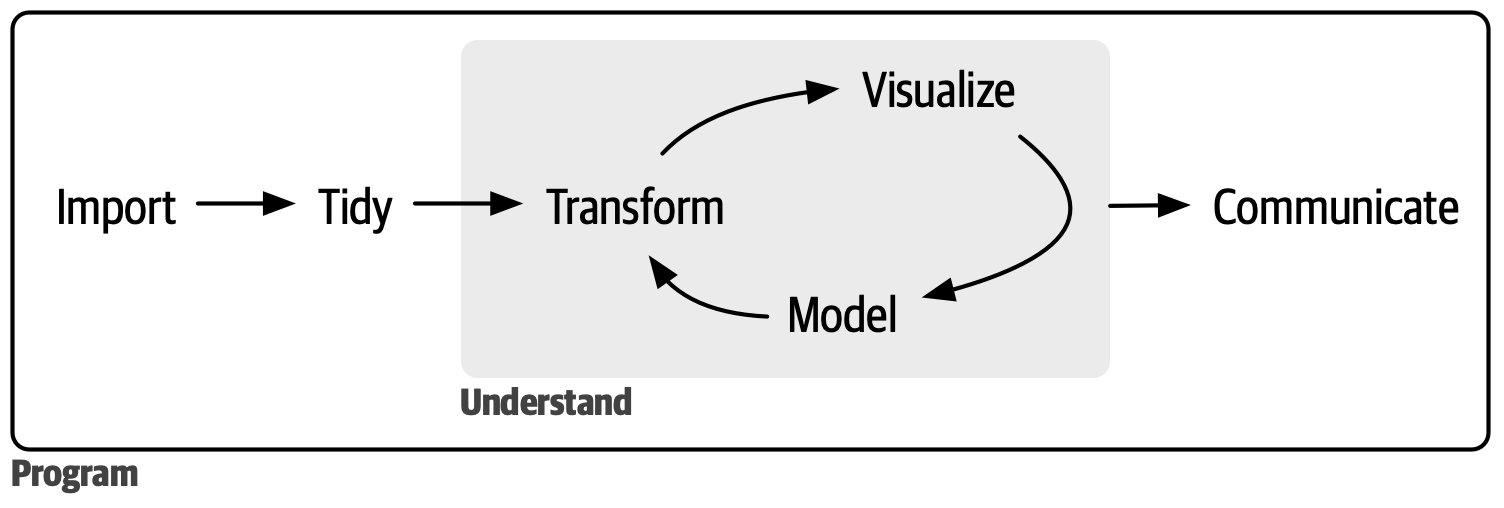
\includegraphics[width=6.5in,height=\textheight,keepaspectratio]{images/r4ds_data_science_cicle.png}

  }

  \caption{Data science cicle (\citeproc{ref-wickham_r_2023}{Wickham et
  al., 2023})}

  \end{figure}%
\item
  NLP: Vajjala et al. (\citeproc{ref-vajjala_practical_2020}{2020}):
  tasks such as ``text classification, information extraction,
  information retrieval, conversational agent, text summarization,
  question anserwing, machine translation''

  \begin{figure}[H]

  {\centering 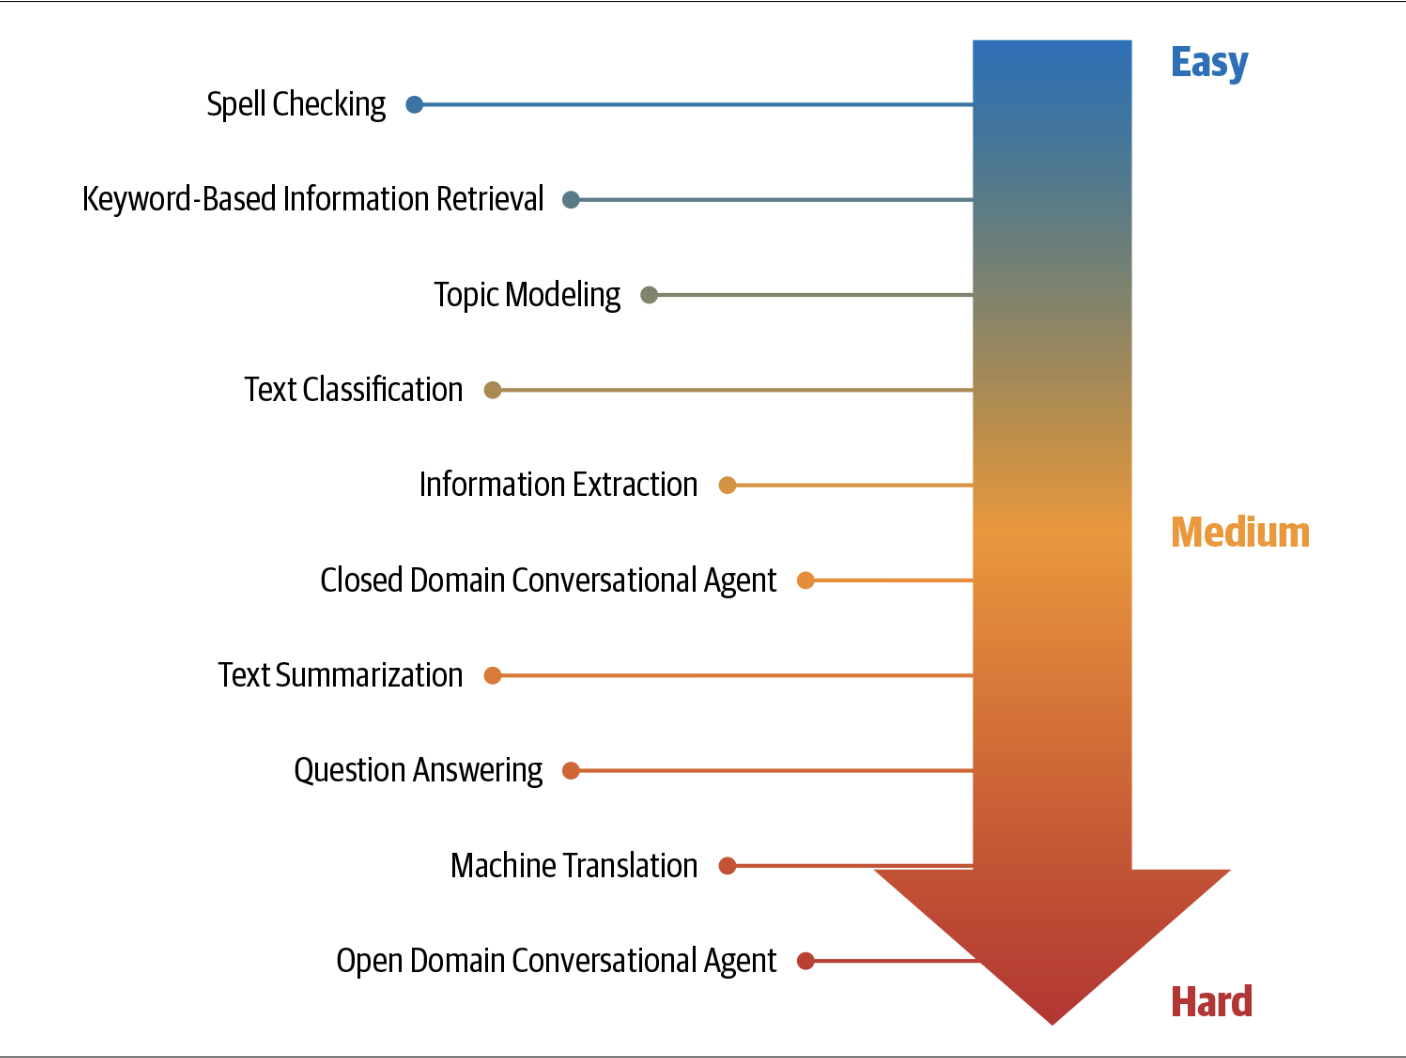
\includegraphics[width=4.59375in,height=\textheight,keepaspectratio]{images/vajjala-2020_nlp_complexity.png}

  }

  \caption{`NLP tasks organized according to their relative difficulty'
  (\citeproc{ref-vajjala_practical_2020}{Vajjala et al., 2020})}

  \end{figure}%
\item
  LLMs: `ushered in a new era for natural language processing (NLP)';
  ``are deep neural networks models; developed over the past few
  years'', `NLP models performed well in many tasks' -- they focused on
  specific tasks; `failed on follow complex instructions, contextual
  analysis and creating coherent and contextually appropriate original
  text'. Raschka (\citeproc{ref-raschka_build_2024}{2024})
\item
  chose sota models, both commercial and open source
\item
  gathered data, cleaned and adapted: Lacerda e Silva
  (\citeproc{ref-lacerda_e_silva_punindo_2021}{2021})
\item
  design a prompt to extract the same features, according with Lacerda e
  Silva's dictionary. prompting relies on the ability of the model
  `understand' specific instructions and act accordingly. So with
  several iterations, it was possible to guide the model on how to
  perform the task
\item
  run models
\item
  fine tuned
\item
  test again
\item
  deep dive in the results
\end{itemize}

* method: - gathered data from judicial sentences in São Paulo -
received access from dataset from Lacerda: ± 400 judicial sentences
labelled - cleaned data - prompt engeneering - used commercial OS
(OpenAI) as baseline - tryied the OS models - llama - gemma - tucano -
lawma - lola - libraries HF and unsloth - ft models - compared their
performance - limitations: - drug traffic, sao paulo - 2017/2018 - only
models that were possible to access - small sample to ft and test -
tucano, lawma: - context window was too short to legal docs; - tried
with no success to apply rope scaling or yarn - tried RAG to retrieve
relevant parts; tried rag to squish the text - possibility: try a
task-based prompt -- still limited window, but might be sufficient to
many documents - lack of computational resources

\section{Data Sources}\label{data-sources}

\begin{itemize}
\tightlist
\item
  \textbf{Lacerda Dataset}: Lacerda e Silva
  (\citeproc{ref-lacerda_e_silva_punindo_2021}{2021}) A comprehensive
  empirical analysis was conducted on over 400 legal cases related to
  drug trafficking. The researcher collected these cases from the São
  Paulo State Court of Justice (TJSP), focusing on a sample that covered
  the years 2017 and 2018. Approximately 35 features were manually
  annotated and labeled for each case. Access to the dataset was
  obtained by contacting the researcher, who provided it for further
  adaptation to meet the specific requirements of this research. Some of
  the original features also referred to other documents rather than the
  judicial decision, and, therefore, they were excluded (since it would
  not be reasonable that the model inferred that). Features related to
  biological data were also excluded for ethical reasons.
\end{itemize}

Also, I have tried to access Instituto de Pesquisa Econômica Aplicada
(Ipea) \& Brasil. Ministério da Justiça e Segurança Pública
(\citeproc{ref-instituto_de_pesquisa_economica_aplicada_ipea_perfil_2023}{2023})
micro data to build a golden dataset since they have about 3.5k data
points labelled. I have filled a freedom of information request and,
although it was possible to access the
\href{https://www.gov.br/mj/pt-br/assuntos/sua-protecao/politicas-sobre-drogas/pesquisa-e-informacao-3/pesquisa\%20IPEA/pesquisa-ipea-perfil-processado-e-producao-de-provas}{general
dataset}, they have not provided the lawsuit identifier, so it was not
possible to match each row in their dataset to a legal case and,
therefore, to a specific document.

\begin{itemize}
\item
  \textbf{Judicial Decisions}: The documents relative to each decision
  case analyzed by the Lacerda Dataset were extracted automatically from
  the TJSP website. Since there is no API to that, the process was done
  using Filho \& Trecenti (\citeproc{ref-filho_coleta_2020}{2020})
  package called \{tjsp\}. It gathered metadata of each case and the
  decision in string format in an R data frame. Some cases were
  collected by its .pdf files and read automatically.
\item
  \textbf{Final dataset}: After cleaning, some duplications were
  excluded, and some documents were not collected; the final result was
  a dataset with 258 cases. Also, the final dataset contained 50
  columns, which was due to some categorical features being transformed
  into a boolean. For instance, the column \emph{DenDrogas} contained
  information about the most common articles of Law in the accusation.
  It was transformed into the columns \emph{denuncia\_art\_33},
  \emph{denuncia\_art\_34}, and \emph{denuncia\_art\_35}.
\item
  data from legal experts -- Lacerda e Silva
  (\citeproc{ref-lacerda_e_silva_punindo_2021}{2021})
\end{itemize}

\section{Methods}\label{methods}

-- different tasks, that's why NLP technichs were not feasible --
Vajjala et al. (\citeproc{ref-vajjala_practical_2020}{2020}):
``Recently, large transformers have been used for transfer learning with
smaller down‐stream tasks. Transfer learning is a technique in AI where
the knowledge gained while solving one problem is applied to a different
but related problem. With transformers, the idea is to train a very
large transformer mode in an unsupervised manner (known as pre-training)
to predict a part of a sentence given the rest of the content so that it
can encode the high-level nuances of the language in it.''
--\textgreater{} pick some basemodel and use it to the specific task

-- not enought to have an answer, it should be an structured output:
JSON. force the output to match a json-style was a challenge, which were
overcome with Chase (\citeproc{ref-chase_langchain_2022}{2022}).
commercial models are better on this, and do this with the open-source
was a challenge

-- context window: at least 16k is needed; were insufficient. tryied
rope-scaling and yarn but lacked computational resources. Daniel Han \&
team (\citeproc{ref-daniel_han_unsloth_2023}{2023}) was a good and
functional option, but it only worked with newer infrastructure.

-- Raschka (\citeproc{ref-raschka_build_2024}{2024}), Lora -- Daniel Han
\& team (\citeproc{ref-daniel_han_unsloth_2023}{2023}) enabled using the
models

We used 12 models in this research. OpenAI models were considered
commercial, and the others were open source. Also, OpenAI does not
disclose its architectures, so it is impossible to know its number of
parameters beforehand.

\begin{itemize}
\tightlist
\item
  etl
\item
  prompt engeneenering, build schema
\item
  generation in OpenAI's models
\item
  evaluation pipeline
\item
  generation with commercial models

  \begin{itemize}
  \tightlist
  \item
    window context: rope scaling, yarn, rag, chuncking
  \item
    structured output
  \item
    base model generation
  \end{itemize}
\item
  finetune commercial and open source models

  \begin{itemize}
  \tightlist
  \item
    OpenAI's API
  \item
    Unsloth
  \end{itemize}
\item
  final evaluation
\end{itemize}

\begin{longtable}[t]{llll}

\toprule
model & family & parameters & type\\
\midrule
GPT 4.1 & OpenAI & unknown & commercial\\
GPT 4.1-mini & OpenAI & unknown & commercial\\
GPT 4.1-nano & OpenAI & unknown & commercial\\
GPT 4o & OpenAI & unknown & commercial\\
GPT 4o-mini & OpenAI & unknown & commercial\\
\addlinespace
o3-mini & OpenAI & unknown & commercial\\
Gemma 3 & Gemma & 27 B & open-source\\
Gemma 3 & Gemma & 12 B & open-source\\
Gemma 3 & Gemma & 1 B & open-source\\
Llama 3.1 & Llama & 8 B & open-source\\
\addlinespace
Llama 3.2 & Llama & 3 B & open-source\\
Phi 4 & Phi & 14 B & open-source\\
Lawma 8B & Lawma & 8 B & open-source\\
Tucano & Tucano & 2.4 B & open-source\\
\bottomrule


\caption{\label{tbl-metadata}Basemodels used}

\tabularnewline
\end{longtable}

\section{Limitations}\label{limitations}

-- little samples, altough high quality -- only used one field of law,
only São Paulo -- prompt very large -- might be some overfitting --

\bookmarksetup{startatroot}

\chapter{Results}\label{results}

\begin{figure}[H]

{\centering 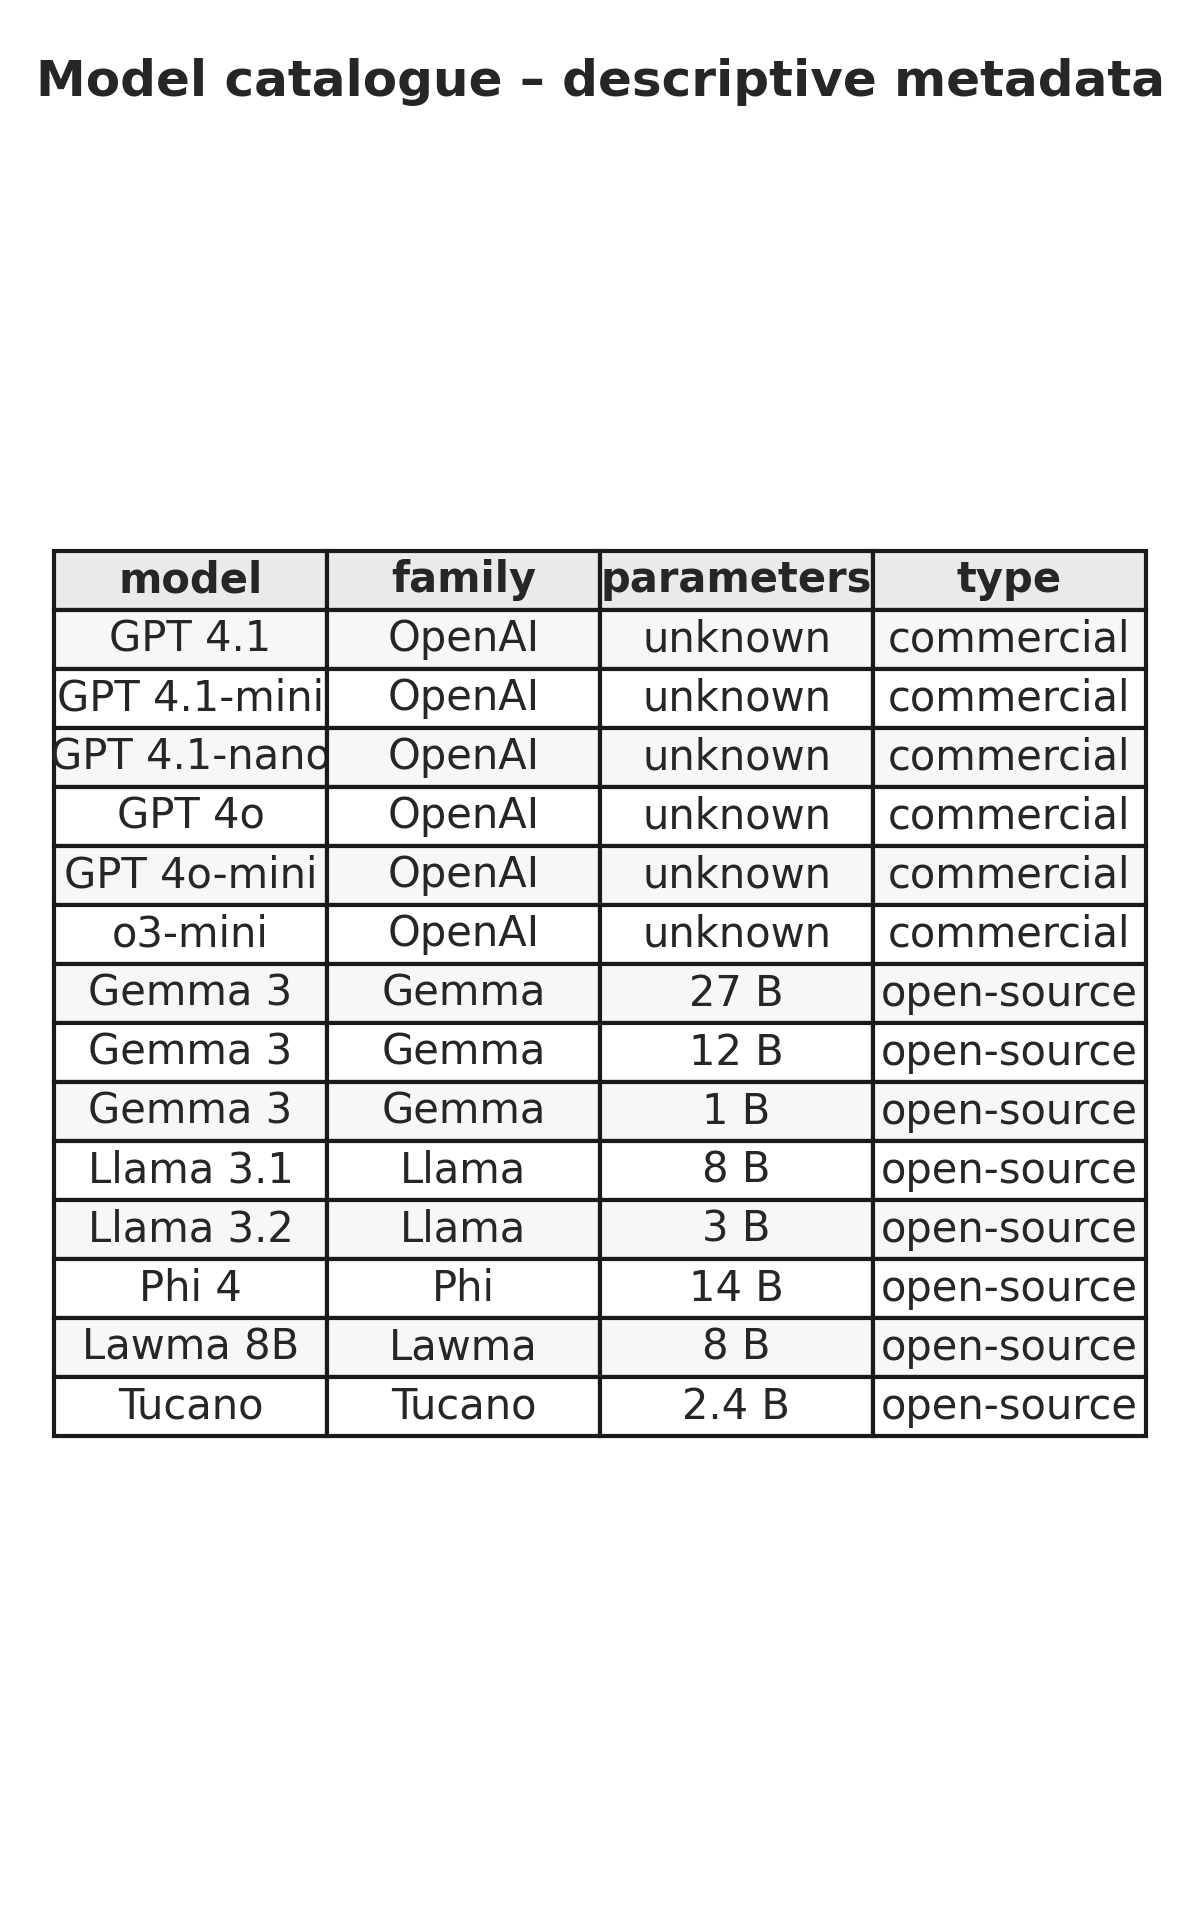
\includegraphics[width=1\linewidth,height=\textheight,keepaspectratio]{../../evaluate_results/model_metadata_table.png}

}

\caption{fig1}

\end{figure}%

bla bla

\begin{figure}[H]

{\centering \pandocbounded{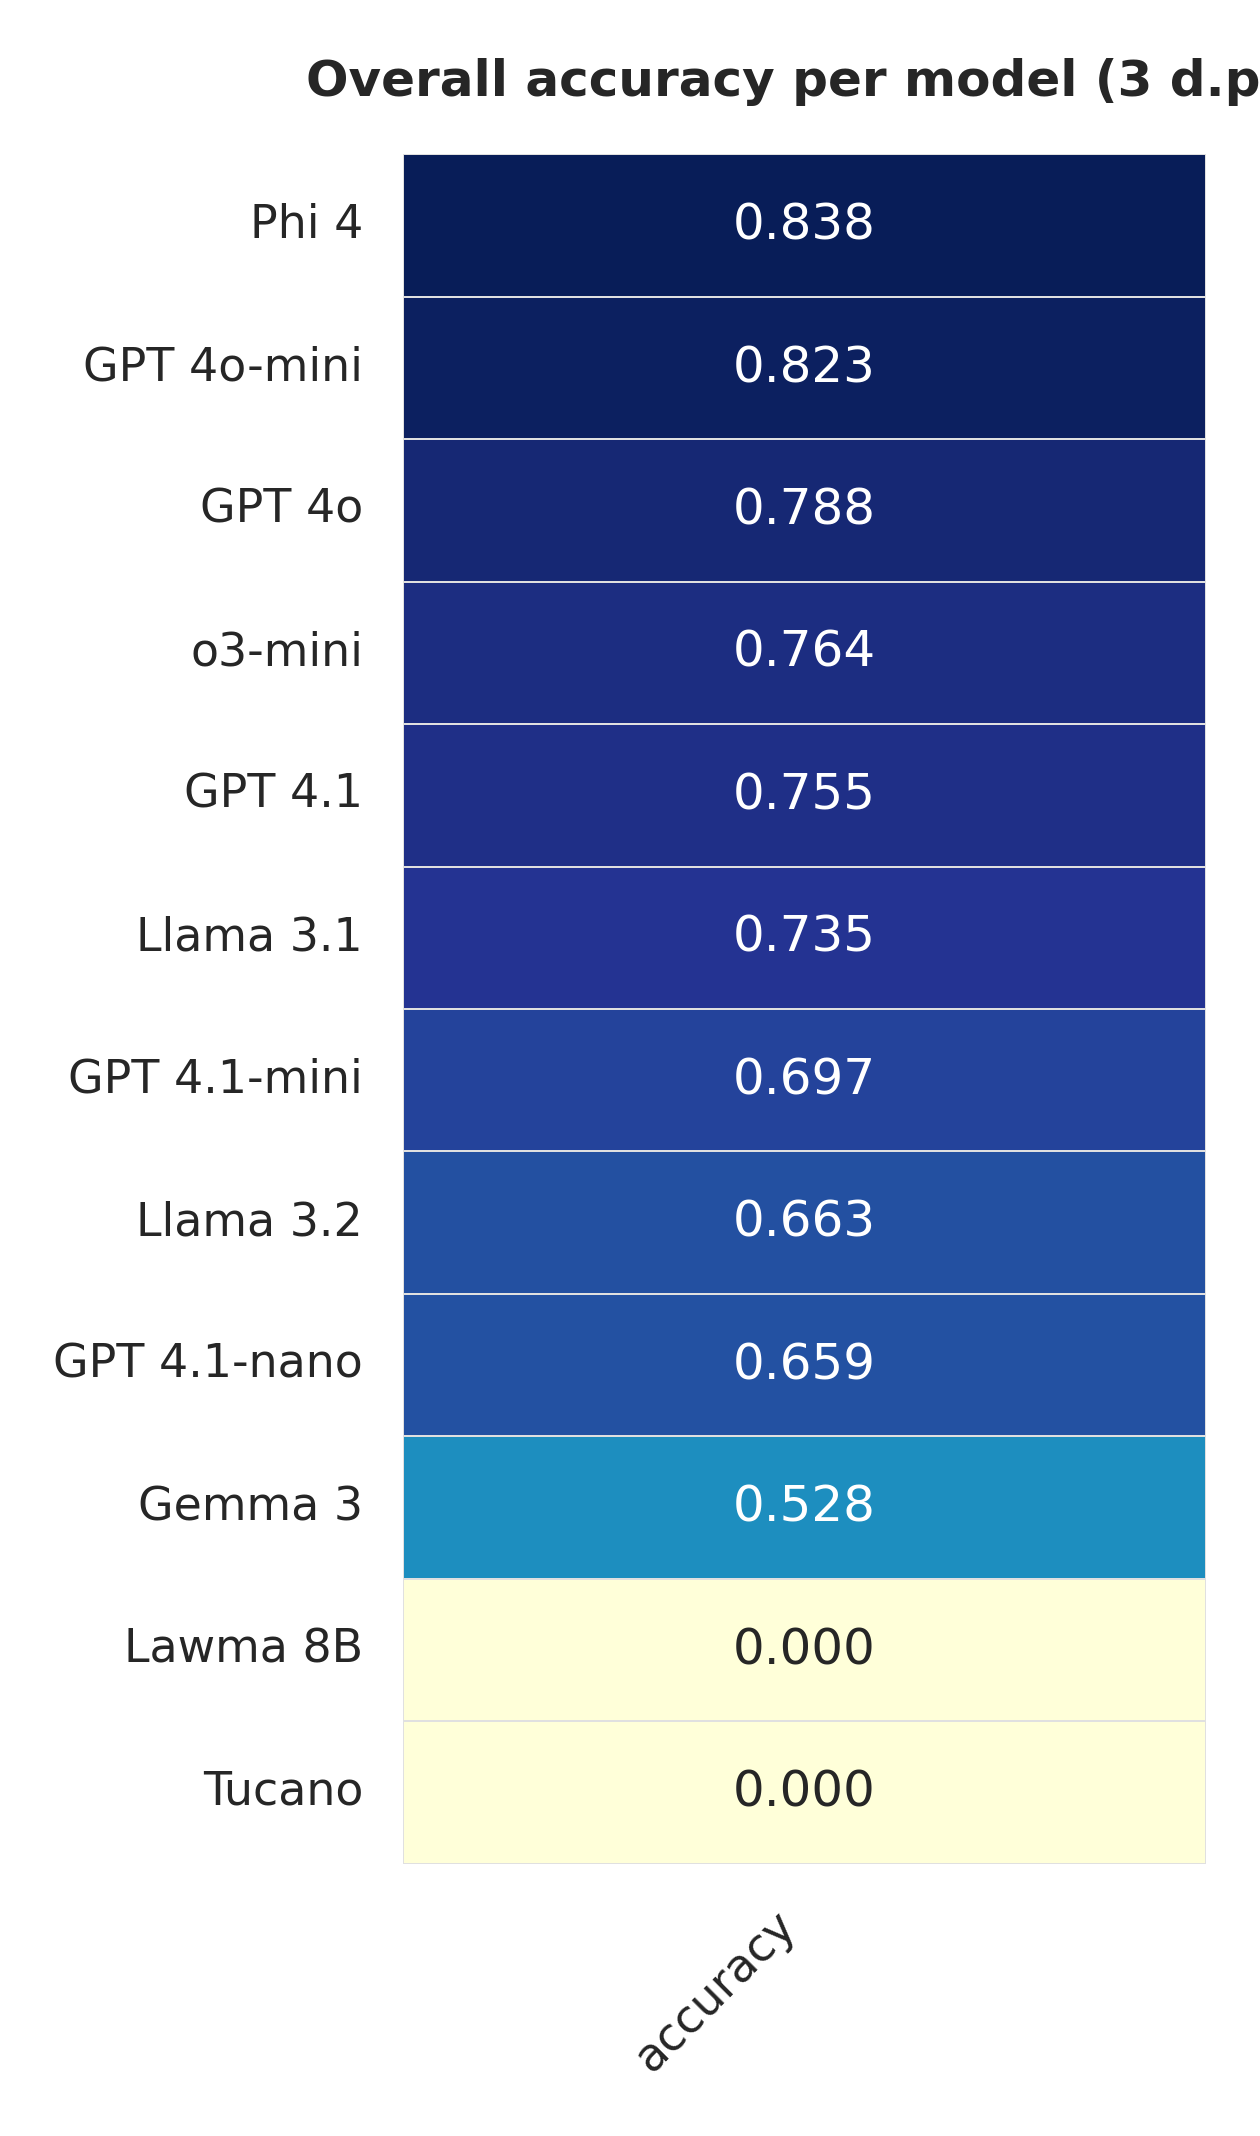
\includegraphics[keepaspectratio]{../../evaluate_results/accuracy_heatmap.png}}

}

\caption{fig2}

\end{figure}%

bla bla

\begin{figure}[H]

{\centering \pandocbounded{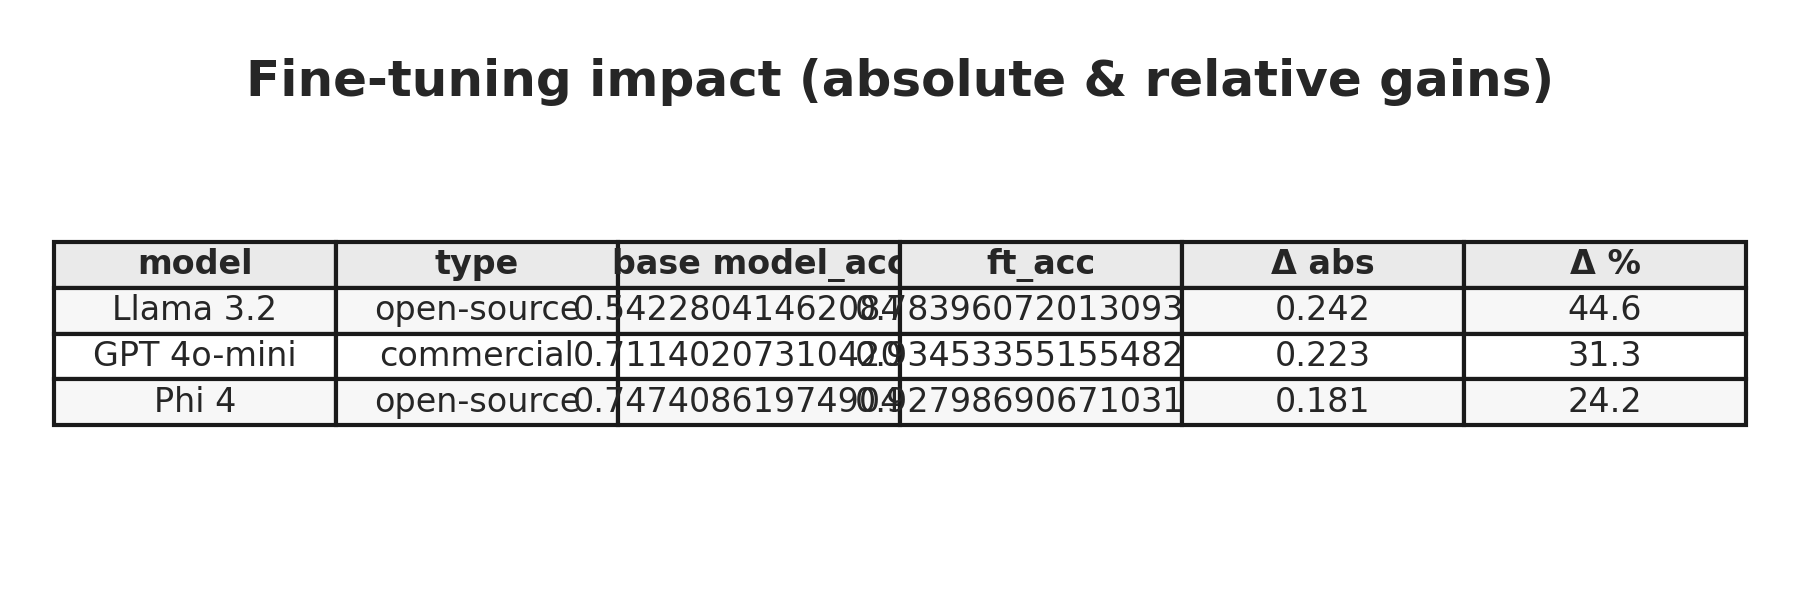
\includegraphics[keepaspectratio]{../../evaluate_results/finetune_impact_table.png}}

}

\caption{fig3}

\end{figure}%

After 17 experiments\footnote{Ignoring validation tests and the
  experiences to try to overcome the limitations regarding context
  windows. Also, in this count there were the fine tune.}, the metrics
above regarding accuracy were gathered. By accuracy, we are considering
the proportion of exact answers relative to the total answers. Below, we
can see the performance of the base models before fine-tuning.

\begin{longtable}[t]{llllr}

\toprule
family & type & model & parameters & accuracy\\
\midrule
Gemma & open-source & Gemma 3 & 27 B & 0.8200\\
OpenAI & commercial & GPT 4o & unknown & 0.7878\\
OpenAI & commercial & o3-mini & unknown & 0.7638\\
Gemma & open-source & Gemma 3 & 12 B & 0.7627\\
OpenAI & commercial & GPT 4.1 & unknown & 0.7545\\
\addlinespace
Phi & open-source & Phi 4 & 14 B & 0.7474\\
Llama & open-source & Llama 3.1 & 8 B & 0.7354\\
OpenAI & commercial & GPT 4o-mini & unknown & 0.7114\\
OpenAI & commercial & GPT 4.1-mini & unknown & 0.6967\\
OpenAI & commercial & GPT 4.1-nano & unknown & 0.6590\\
\addlinespace
Llama & open-source & Llama 3.2 & 3 B & 0.5423\\
Gemma & open-source & Gemma 3 & 1 B & 0.0000\\
\bottomrule


\caption{\label{tbl-accuracy-metadata}Accuracy of base models}

\tabularnewline
\end{longtable}

The model Gemma 3-1B achieved 0.0 accuracy due to its inability to yield
valid structured JSON outputs.

The model that best performed in a zero-shot approach was the Gemma
3-27B parameters, which, surprisingly, also beat the benchmark
commercial models, even GPT-4o. Also, the Gemma 3 family likely yields
accurate results since the lighter version with the 12B parameter
performed very well and was better than the newly released GPT-4.1. The
model Phi-4 also performed very well, betting OpenAI's smaller models.
Regarding the Llama family, the 3.1 version performed better than the
4o-mini and the smaller GPT 4.1-mini and GPT 4.1-nano. On the other
hand, Llama 3.2 had a bad performance.

Trying to understand a more fine-grained analysis, breaking the results
by the kind of tasks was possible. The \emph{numeric} tasks are those
related to extracting and calculating the amount of drugs or prison time
in months: those tasks involved not only recognizing the numbers
(entities) but also `calculating' the final value. The \emph{boolean}
tasks are generally in the realm of question answering in a
TRUE/FALSE/None style (for instance, if art. 33 was the basis of the
sentence or if there were confessions by the defendant). The
\emph{categorical} tasks are those closely related to classification
tasks, such as the case's outcome (conviction, acquittal, etc.). The
\emph{open textual} tasks are more likely to be similar to named entity
recognition: the name of the Judge and the defendant in this case.

\begin{figure}

\centering{

\pandocbounded{
\includegraphics[keepaspectratio]{../../evaluate_results/task_accuracy_heatmap.png}}

}

\caption{\label{fig-base_model}Tasks by accuracy}

\end{figure}%

We can see that the \emph{open textual} tasks have a very high level of
performance in nearly all models, while the \emph{boolean} and
\emph{categorical} tasks were more diverse performance-wise. We can also
see some differences in numeric tasks, but in general, they all
performed very well.

Those results suggested that continuing to work with open-source models
was a promising strategy. So, fine-tuning was performed with the models
OpenAI 4o-mini (which is the recommended model by OpenAI), Llama 3.2
(3B), and Phi4. No resources were available to perform fine-tuning on
other models. After the fine-tuning, we could see a big improvement in
the results.

\begin{figure}

\centering{

\pandocbounded{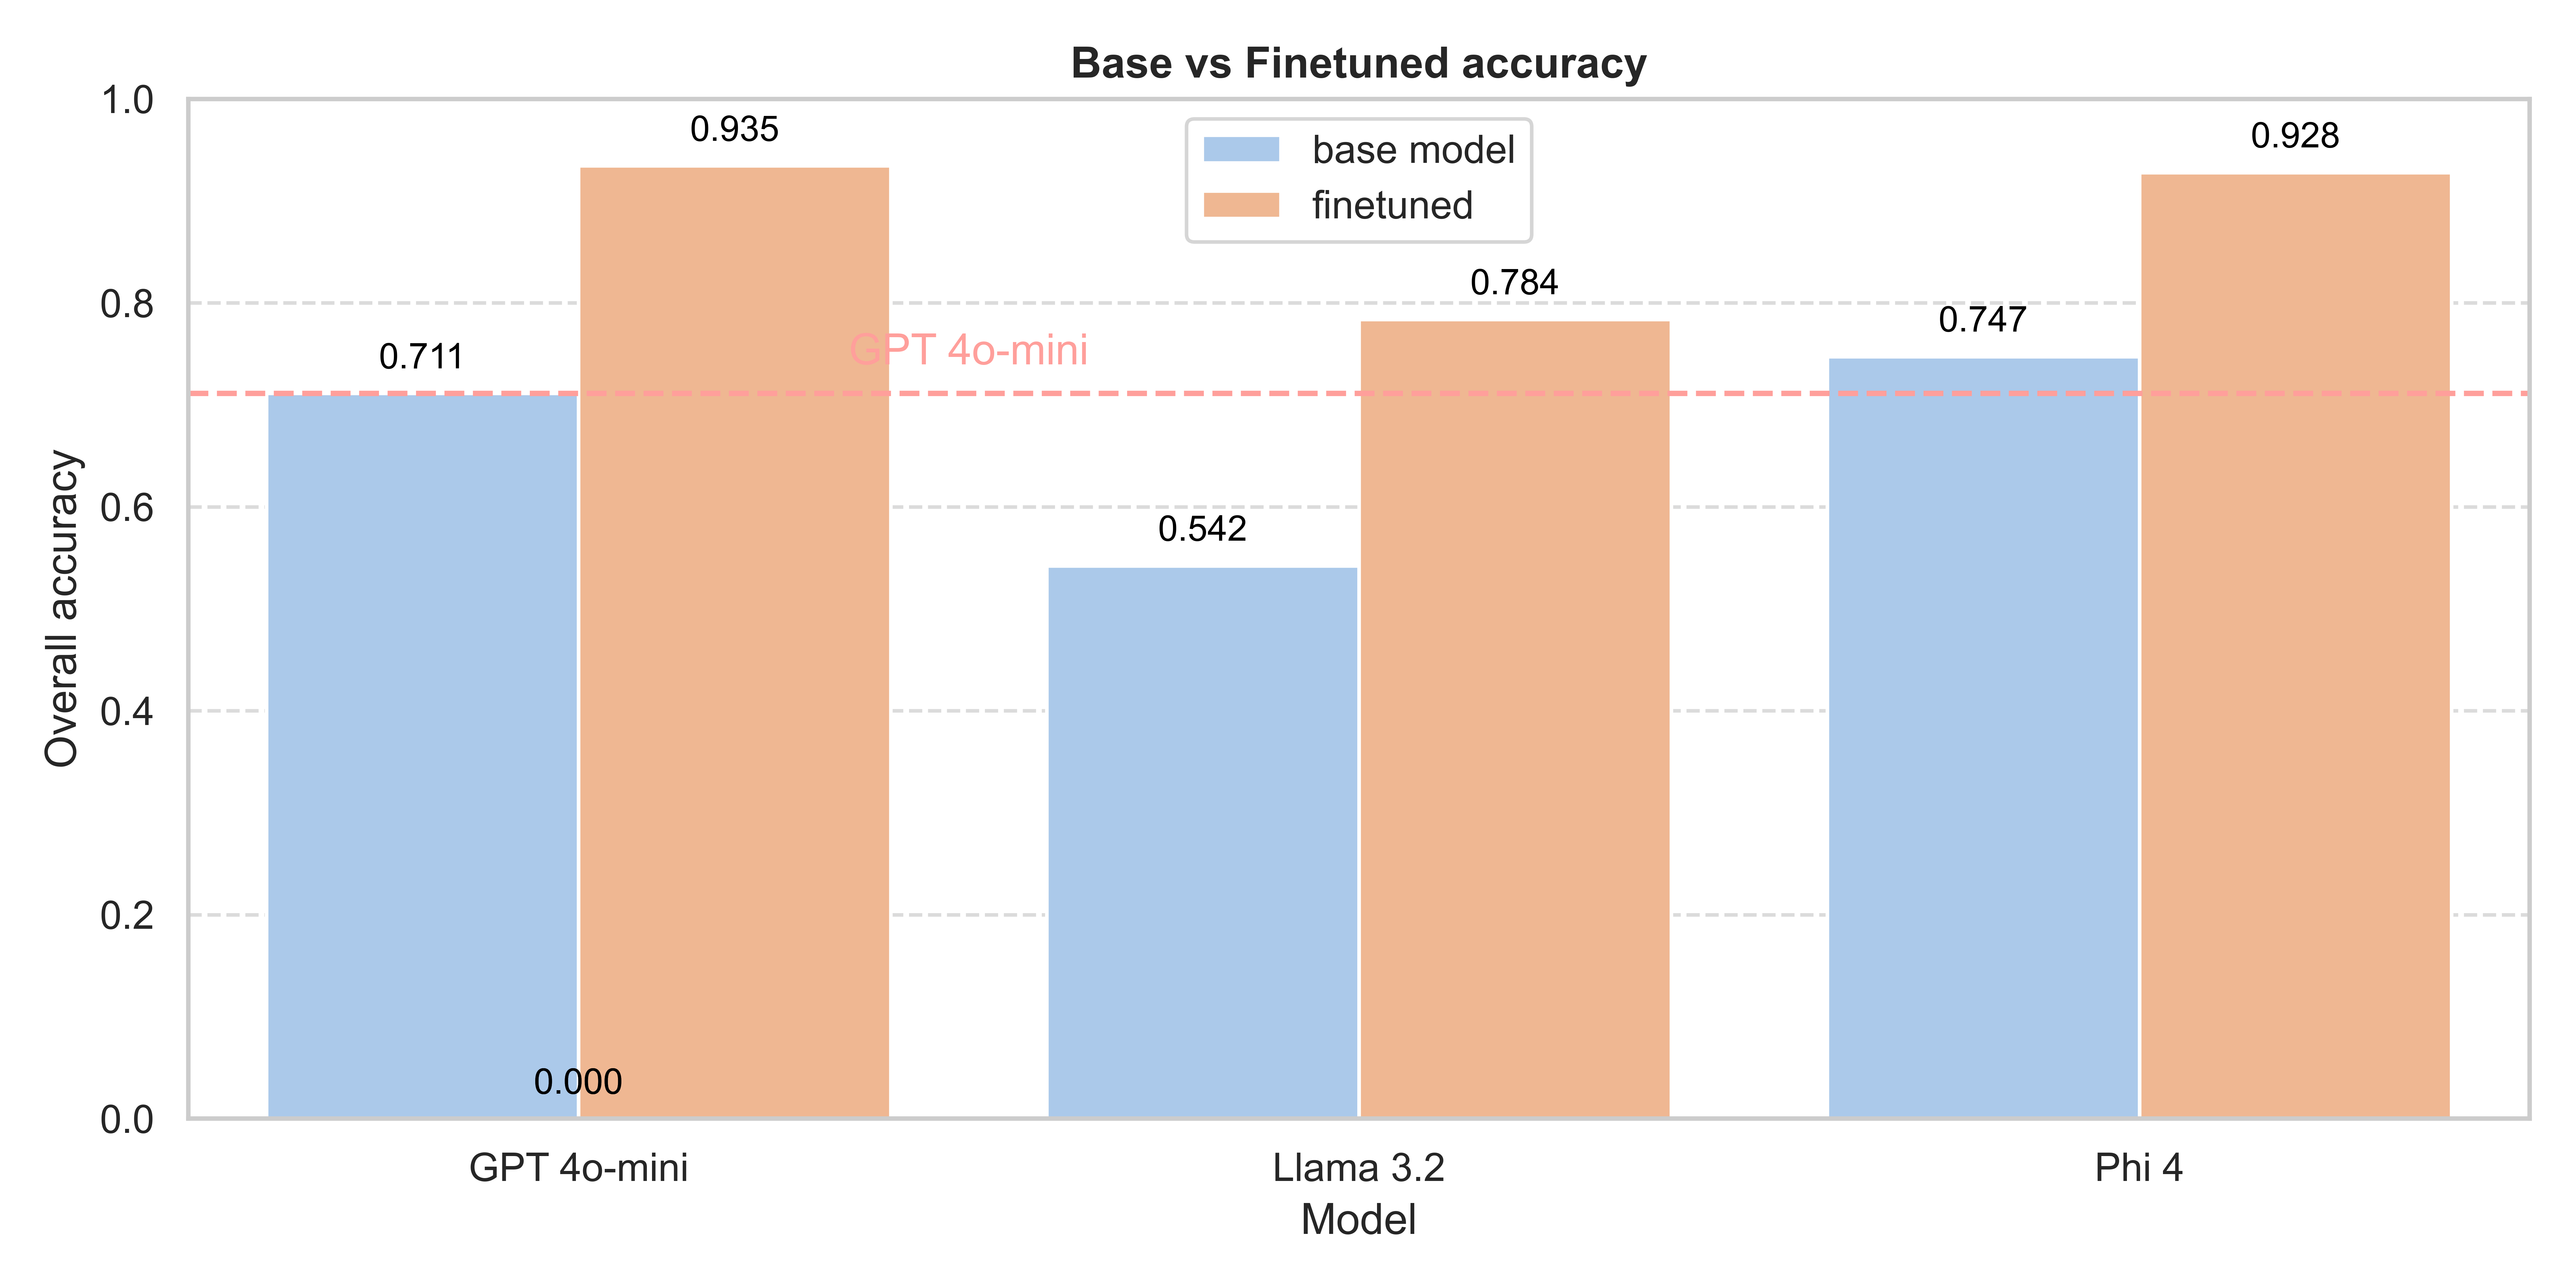
\includegraphics[keepaspectratio]{../../evaluate_results/base_vs_finetuned_accuracy.png}}

}

\caption{\label{fig-finetune}Models after fine-tuning}

\end{figure}%

The process of fine-tuning, even with a small dataset with 186 cases,
highly improved the performance of the models, confirming the `power of
specialization' as suggested by Dominguez-Olmedo et al.
(\citeproc{ref-dominguez-olmedo_lawma_2024}{2024}). As
Figure~\ref{fig-finetune} showed, model Phi4 tied with GPT 4o-mini and
the much smaller Llama 3.2 (3B) learned very easily, even with both
models being trained with the same 10 epochs. With a richer dataset
and/or more epochs, it would be possible to reach or even surpass GPT
4o-mini performance.

\begin{longtable}[t]{lrrr}

\toprule
metric & GPT 4o-mini & Llama 3.2 & Phi 4\\
\midrule
Δ accuracy & 0.22 & 0.24 & 0.18\\
\% accuracy & 31.37 & 44.57 & 24.16\\
Δ boolean & 0.29 & 0.20 & 0.21\\
\% boolean & 43.56 & 34.54 & 28.63\\
Δ categorical & -0.04 & 0.48 & 0.14\\
\addlinespace
\% categorical & -4.46 & 145.31 & 17.76\\
Δ numeric & 0.11 & 0.28 & 0.09\\
\% numeric & 14.44 & 62.15 & 11.17\\
Δ open textual & 0.01 & 0.21 & 0.08\\
\% open textual & 1.35 & 33.00 & 8.82\\
\bottomrule


\caption{\label{tbl-finetune-delta}Fine tuned models: change in accuracy
(absolute value Δ and relative value \%)}

\tabularnewline
\end{longtable}

As Table~\ref{tbl-finetune-delta} shows, Llama 3.2(3B) had the most
significant change in its performance, especially with the categorical
tasks. Specifically, with this task, we could see a performance
degradation of GPT 4o-mini. Phi4, \footnote{There is the
  \href{https://huggingface.co/microsoft/Phi-4-mini-instruct}{mini
  version of Phi-4}, however it was not possible to run or fine-tune it
  with the actual computational resources.} though they had the
second-best performance, learned less than Llama, which suggests a
ceiling. Assuming that, in those architectures, the number of parameters
is the critical factor, fewer parameters than 14B and more than 3B would
be ideal.

\bookmarksetup{startatroot}

\chapter{Discussion}\label{discussion}

Lorem ipsum dolor sit amet, consectetur adipiscing elit

\section{Key Findings}\label{key-findings}

\begin{itemize}
\tightlist
\item
  results - os: - cons: difficult to manage, several have short context
  window; computationaly intensive; - pro: privacy; costs; fast paced;
  adaptability; full control; - comercial: - cons: privacy; costs; -
  pro: reliability; easiness; credibility - indeed, specialization is a
  good strategy - have good potential, altough more testing is needed
\end{itemize}

\section{Future Research}\label{future-research}

\begin{verbatim}
- future research:
  - quantization; prunning; distillation;
  - task-based approach
\end{verbatim}

\section{Policy Recommendations}\label{policy-recommendations}

\begin{itemize}
\item
  Academia: Disclose data from empirical legal research as much as
  possible, as it would be a valuable resource for fine-tuning models.
  If IPEA released the data from Instituto de Pesquisa Econômica
  Aplicada (Ipea) \& Brasil. Ministério da Justiça e Segurança Pública
  (\citeproc{ref-instituto_de_pesquisa_economica_aplicada_ipea_perfil_2023}{2023}),
  would it be possible to achieve even better results.
\item
  Open source community: keep at least 128k context window standard and
  develop light open-source models. Wolf et al.
  (\citeproc{ref-wolf_transformers_2020}{2020}) is a fundamental
  framework for training and inference. Daniel Han \& team
  (\citeproc{ref-daniel_han_unsloth_2023}{2023}) was valuable in
  fine-tuning models efficiently.
\item
  Judiciary branch: should ensure that data and documents from lawsuits
  are available digitally for research while maintaining high standards
  of privacy. Anonymization would make this feasible.
\item
  Instituions interested in empirical legal research: OpenAI's API
  probably offers a better balance of ease and performance. However,
  open-source models have proven powerful for these tasks and might be
  deployed to accelerate empirical research in Law.
\item
  Law schools: invest in data literacy for legal students and
  practitioners.
\end{itemize}

\section{Conclusion}\label{conclusion}

\begin{verbatim}
* conclusions:
  - llms are good tools to leverage empirical legal research in BR
  - commercial models: still up to date a good strategy, despite of its costs and privacy issues
    - pre-process to anonymize is an option
  - os models: feasible and decent baseline performances in certain models; ft is a good strategy that increases a lot performance
\end{verbatim}

Alva-Manchego et al.
(\citeproc{ref-alva-manchego_suitability_2021}{2021})

Lorem ipsum dolor sit amet, consectetur adipiscing elit.

\bookmarksetup{startatroot}

\chapter{References}\label{references}

Lorem ipsum dolor sit amet, consectetur adipiscing elit.

\phantomsection\label{refs}
\begin{CSLReferences}{1}{0}
\bibitem[\citeproctext]{ref-almeida_sabia-2_2024}
Almeida, T. S., Abonizio, H., Nogueira, R., \& Pires, R. (2024).
\emph{Sabiá-2: {A} {New} {Generation} of {Portuguese} {Large} {Language}
{Models}}. arXiv. \url{https://doi.org/10.48550/arXiv.2403.09887}

\bibitem[\citeproctext]{ref-alva-manchego_suitability_2021}
Alva-Manchego, F., Scarton, C., \& Specia, L. (2021). The
({Un}){Suitability} of {Automatic} {Evaluation} {Metrics} for {Text}
{Simplification}. \emph{Computational Linguistics}, \emph{47}, 861--889.
\url{https://doi.org/10.1162/coli_a_00418}

\bibitem[\citeproctext]{ref-alves_da_silva_aspectos_2022}
Alves da Silva, P. E. (2022). Aspectos metodológicos da pesquisa
empírica em {Direito} com processos judiciais físicos e eletrônicos. In
\emph{Estudos empíricos em processo e organização judiciária}. Expert.

\bibitem[\citeproctext]{ref-associacao_brasileira_de_jurimetria_avaliacao_2019}
Associação Brasileira de Jurimetria. (2019). \emph{Avaliação do
{Impacto} de {Critérios} {Objetivos} na {Distinção} {Entre} {Posse} para
{Uso} e {Posse} para {Tráfico}: {Um} estudo {Jurimétrico}}. Associação
Brasileira de Jurimetria.
\url{https://abj.org.br/pdf/20190402_abj_criterios_objetivos.pdf}

\bibitem[\citeproctext]{ref-bertalan_predicting_nodate}
Bertalan, V. G. F., \& Ruiz, E. E. S. (n.d.). \emph{Predicting
{Judicial} {Outcomes} in the {Brazilian} {Legal} {System} {Using}
{Textual} {Features}}.

\bibitem[\citeproctext]{ref-cabrera_de_bonito_pesquisa_2025}
Cabrera De Bonito, B., Veloso De Castro, C., \& Korasaki, V. (2025).
{PESQUISA} {QUANTITATIVA} {NO} {DIREITO}: {UMA} {REVISÃO}
{BIBLIOGRÁFICA}. \emph{Revista de Estudos Empíricos Em Direito},
\emph{11}. \url{https://doi.org/10.19092/reed.v11.830}

\bibitem[\citeproctext]{ref-chase_langchain_2022}
Chase, H. (2022). \emph{{LangChain}}.
\url{https://github.com/langchain-ai/langchain}

\bibitem[\citeproctext]{ref-chen_empowering_2025}
Chen, W. (2025). Empowering innovation: {The} next generation of the
{Phi} family. In \emph{Microsoft Azure Blog}.
\url{https://azure.microsoft.com/en-us/blog/empowering-innovation-the-next-generation-of-the-phi-family/}

\bibitem[\citeproctext]{ref-correa_tucano_2024}
Corrêa, N. K., Sen, A., Falk, S., \& Fatimah, S. (2024). \emph{Tucano:
{Advancing} {Neural} {Text} {Generation} for {Portuguese}}. arXiv.
\url{https://doi.org/10.48550/arXiv.2411.07854}

\bibitem[\citeproctext]{ref-costa_eficacia_2011}
Costa, S. H. da, Silva, P. E. A. da, Sabino, M. A. da C., Fernandes, D.
C. M., \& Lusvarghi, L. A. dos S. (2011). \emph{A eficácia do sistema
jurídico de prevenção e combate à improbidade administrativa}
{[}Publicação de relatório de pesquisa{]}. Secretaria de Assuntos
Legislativos do Ministério da Justiça.
\url{https://web.archive.org/web/20211004195943/http://pensando.mj.gov.br/wp-content/uploads/2015/07/34Pensando_Direito1.pdf}

\bibitem[\citeproctext]{ref-daniel_han_unsloth_2023}
Daniel Han, M. H., \& team, U. (2023). \emph{Unsloth}.
\url{http://github.com/unslothai/unsloth}

\bibitem[\citeproctext]{ref-dominguez-olmedo_lawma_2024}
Dominguez-Olmedo, R., Nanda, V., Abebe, R., Bechtold, S., Engel, C.,
Frankenreiter, J., Gummadi, K., Hardt, M., \& Livermore, M. (2024).
\emph{Lawma: {The} {Power} of {Specialization} for {Legal} {Tasks}}.
arXiv. \url{http://arxiv.org/abs/2407.16615}

\bibitem[\citeproctext]{ref-dornelles_o_2021}
Dornelles, R. F. (2021). O {STF}, o controle concentrado e a pandemia.
In \emph{Associação Brasileira de Jurimetria}.
\url{https://lab.abj.org.br/posts/2021-04-13-stf-controle-concentrado/}

\bibitem[\citeproctext]{ref-filho_coleta_2020}
Filho, J. de J., \& Trecenti, J. (2020). \emph{Coleta e organização de
dados do {Tribunal} de {Justiça} de {São} {Paulo}}.
\url{https://jjesufilho.github.io/tjsp/}

\bibitem[\citeproctext]{ref-instituto_de_pesquisa_economica_aplicada_ipea_perfil_2023}
Instituto de Pesquisa Econômica Aplicada (Ipea), \& Brasil. Ministério
da Justiça e Segurança Pública. (2023). \emph{Perfil do processado e
produção de provas nas ações criminais por tráfico de drogas : Relatório
analítico nacional dos {Tribunais} {Estaduais} de {Justiça} {Comum}}.
Instituto de Pesquisa Econômica Aplicada (Ipea).
\url{https://doi.org/10.38116/ri221151}

\bibitem[\citeproctext]{ref-junior_juru_2024}
Junior, R. M., Pires, R., Romero, R., \& Nogueira, R. (2024).
\emph{Juru: {Legal} {Brazilian} {Large} {Language} {Model} from
{Reputable} {Sources}}. arXiv.
\url{https://doi.org/10.48550/arXiv.2403.18140}

\bibitem[\citeproctext]{ref-katz_natural_2023}
Katz, D. M., Hartung, D., Gerlach, L., Jana, A., \& II, M. J. B. (2023).
\emph{Natural {Language} {Processing} in the {Legal} {Domain}}. arXiv.
\url{https://doi.org/10.48550/arXiv.2302.12039}

\bibitem[\citeproctext]{ref-lacerda_e_silva_punindo_2021}
Lacerda e Silva, M. (2021). \emph{Punindo as diferenças: {Gênero}, raça
e geração no sentenciamento de tráfico de drogas na cidade de {São}
{Paulo}}. \url{http://repositorio.unb.br/handle/10482/41413}

\bibitem[\citeproctext]{ref-niklaus_multilegalpile_2023}
Niklaus, J., Matoshi, V., Sturmer, M., Chalkidis, I., \& Ho, D. E.
(2023). \emph{{MultiLegalPile}: {A} {689GB} {Multilingual} {Legal}
{Corpus}}. \url{https://doi.org/10.48550/arXiv.2306.02069}

\bibitem[\citeproctext]{ref-pires_sabia_2023}
Pires, R., Abonizio, H., Almeida, T. S., \& Nogueira, R. (2023).
\emph{Sabiá: {Portuguese} {Large} {Language} {Models}} (Vol. 14197, pp.
226--240). \url{https://doi.org/10.1007/978-3-031-45392-2_15}

\bibitem[\citeproctext]{ref-raschka_build_2024}
Raschka, S. (2024). \emph{Build a {Large} {Language} {Model} (from
{Scratch})}. Manning Publications Co. LLC.
\url{http://ebookcentral.proquest.com/lib/hertie-school/detail.action?docID=31657639}

\bibitem[\citeproctext]{ref-ribeiro_jurimetria_2022}
Ribeiro, E. M. S., Rodello, I. A., \& Morilas, L. R. (2022). Jurimetria:
As possibilidades e os desafios de um modelo para a análise empírica dos
processos e dos atores processuais. In G. M. Gonçalves, R. C. V. Maia,
I. M. Rocha, \& G. P. Teodoro (Eds.), \emph{Estudos empíricos em
processo e organização judiciária}. Editora Expert.
\url{https://experteditora.com.br/wp-content/uploads/2022/02/Estudos-empiricos-em-processo-e-organizacao-judiciaria.pdf}

\bibitem[\citeproctext]{ref-vajjala_practical_2020}
Vajjala, S., Majumder, B., Gupta, A., \& Surana, H. (2020).
\emph{Practical {Natural} {Language} {Processing}: {A} {Comprehensive}
{Guide} to {Building} {Real}-{World} {NLP} {Systems}}. "O'Reilly Media,
Inc.".

\bibitem[\citeproctext]{ref-wickham_r_2023}
Wickham, H., Çetinkaya-Rundel, M., \& Grolemund, G. (2023). \emph{R for
{Data} {Science}} (2nd ed.). O'Reilly Media.
\url{https://r4ds.hadley.nz/}

\bibitem[\citeproctext]{ref-wolf_transformers_2020}
Wolf, T., Debut, L., Sanh, V., Chaumond, J., Delangue, C., Moi, A.,
Cistac, P., Ma, C., Jernite, Y., Plu, J., Xu, C., Le Scao, T., Gugger,
S., Drame, M., Lhoest, Q., \& Rush, A. M. (2020). \emph{Transformers:
{State}-of-the-{Art} {Natural} {Language} {Processing}}. 38--45.
\url{https://www.aclweb.org/anthology/2020.emnlp-demos.6}

\end{CSLReferences}

lorem

\bookmarksetup{startatroot}

\chapter{Acknowledgements}\label{acknowledgements}

Vetor Brasil, ChancenEg. Marina Lacerda Silva, Lynn Kaack, Huy Dang,
Sascha. Prof.~Susana Henriques da Costa, José Jesus Filho, Associação
Brasileira de Jurimetria e Jusbrasil. MDS classes of 2023 and 2025, the
Latin-American Club specially the Brazilians. Special thanks to João
Vitor Krieger, Renan Barbosa. Also, a grateful to Fernanda Horn, Vitor
Moneo, Orisha, Meirelles.

\bookmarksetup{startatroot}

\chapter{Appendix}\label{appendix}

Lorem ipsum dolor sit amet, consectetur adipiscing elit.

\section{List of experiments}\label{list-of-experiments}

\bookmarksetup{startatroot}

\chapter{Appendix I - Lacerda's
Dataset}\label{appendix-i---lacerdas-dataset}

Lorem ipsum

\bookmarksetup{startatroot}

\chapter{Appendix II - Prompt}\label{appendix-ii---prompt}

Lorem ipsum

\bookmarksetup{startatroot}

\chapter{Appendix III - Fine tune
performance}\label{appendix-iii---fine-tune-performance}

Lorem ipsum

\bookmarksetup{startatroot}

\chapter{Appendix IV - Plots and
tables}\label{appendix-iv---plots-and-tables}

Lorem ipsum

\bookmarksetup{startatroot}

\chapter{Appendix V -
Acknowledgments}\label{appendix-v---acknowledgments}


\backmatter


\end{document}
